% USENIX-formatted research paper
% Compile with: pdflatex main && bibtex main && pdflatex main && pdflatex main

\documentclass[letterpaper,twocolumn,10pt]{article}
\usepackage{usenix2019_v3}

\usepackage{graphicx}
\usepackage{booktabs}
\usepackage{amsmath,amssymb}
\usepackage{hyperref}
\usepackage{url}
\usepackage{xcolor}
\usepackage{tikz}
\usetikzlibrary{arrows.meta, positioning, shapes.geometric, fit}

% Compact lists
\usepackage{enumitem}
\setlist{nosep,leftmargin=*}

\begin{document}

% ------------------------------------------------------------------
\title{Verifiable Layer-2 Order Book State:\\ Merkle-Prefix Trees vs.\ Red-Black Trees\\ with Delta-Cached Proof Recovery}

\author{
  {\rm Joshua Kim} \\
  University of Illinois Urbana-Champaign
}

\maketitle

% ------------------------------------------------------------------
% ABSTRACT
% ------------------------------------------------------------------
\begin{abstract}
Layer-2 rollups that host on-chain order books must generate Merkle proofs of state for settlement and dispute resolution.
As order book size grows, proof generation becomes a throughput bottleneck.
We implement and benchmark two authenticated data structures for this role:
a Patricia-compressed Merkle-prefix trie and a hash-augmented Red-Black Tree.
The Merkle-prefix trie generates inclusion proofs in $O(\log N)$ time by collecting sibling hashes along a single root-to-leaf path, while the Red-Black Tree requires an $O(N)$ in-order traversal to build a temporary Merkle commitment before extracting a proof.
To address the orthogonal problem of stale proofs---where concurrent state updates invalidate previously generated proofs---we integrate an Aardvark-style delta cache that patches stale proofs by replaying recorded node-hash changes rather than regenerating proofs from scratch.
Our benchmarks on order books of 100 to 10{,}000 entries show that the Merkle-prefix trie achieves up to 1{,}316$\times$ faster proof generation than the Red-Black Tree at $N = 10{,}000$, and that delta-cache patching recovers stale proofs in roughly 10~$\mu$s regardless of tree size, compared to the ${\sim}9.5$~ms required by full Red-Black Tree proof regeneration.
\end{abstract}

% ------------------------------------------------------------------
% 1  INTRODUCTION
% ------------------------------------------------------------------
\section{Introduction}

Layer-2 (L2) scaling solutions have become essential for high-throughput decentralized exchanges (DEXs) that maintain on-chain order books~\cite{buterin2021rollups, gudgeon2020sok}.
Unlike automated market makers (AMMs), order-book DEXs match limit orders at discrete price levels, requiring the sequencer to maintain a sorted, mutable data structure whose state can be cryptographically committed for settlement on the Layer-1 chain~\cite{starkware2020starkex, dydx2021}.

A critical performance requirement is \emph{proof generation}: producing a Merkle inclusion proof that a given order exists (or has been filled) in the current state.
In optimistic rollups, these proofs are needed for fraud-proof challenges; in validity (ZK) rollups, they feed into the circuit that produces the settlement proof~\cite{kalodner2018arbitrum}.
As the number of active orders $N$ grows, a naive implementation that rebuilds the entire Merkle commitment before extracting a proof imposes an $O(N)$ bottleneck that limits sequencer throughput.

A second, orthogonal challenge is the \emph{stale proof problem}.
In a concurrent L2 system, a proof generated at state version $V$ may become invalid by the time it is consumed at version $V + D$, because intervening mutations have changed the sibling hashes along the proof path.
Regenerating the proof from scratch at version $V + D$ is expensive---especially when the regeneration itself is $O(N)$.

\paragraph{Contributions.}
We present a prototype L2 order book matching engine that addresses both challenges.
Our system compares two authenticated data structures for managing verifiable order book state:
\begin{enumerate}
  \item A \textbf{Patricia-compressed Merkle-prefix trie}~\cite{morrison1968patricia, lighter2023} that generates inclusion proofs in $O(\log N)$ time.
  \item A \textbf{hash-augmented Red-Black Tree}~\cite{cormen2009introduction, bayer1972symmetric} whose structural operations are $O(\log N)$ but whose proof generation requires an $O(N)$ in-order traversal and temporary Merkle tree construction.
\end{enumerate}
To solve the stale proof problem, we integrate an \textbf{Aardvark-style delta cache}~\cite{aardvark2023} that records per-version node-hash changes and patches stale proofs in $O(D \cdot P \cdot C)$ time, where $D$ is the number of versions bridged, $P$ is the proof length, and $C$ is the average number of changed nodes per version.

Our benchmarks demonstrate that:
\begin{itemize}
  \item The Merkle-prefix trie achieves 12$\times$ to 1{,}316$\times$ faster proof generation than the Red-Black Tree across order book sizes of 100 to 10{,}000 entries.
  \item Delta-cache patching recovers stale proofs in ${\sim}10~\mu$s regardless of tree size, versus the ${\sim}9.5$~ms required by Red-Black Tree proof regeneration at $N = 10{,}000$.
  \item The Merkle-prefix trie trades 4--5$\times$ higher memory usage for its proof generation advantage due to Python's dictionary-based trie node representation.
\end{itemize}

\paragraph{Paper outline.}
Section~\ref{sec:related} surveys related work.
Section~\ref{sec:design} describes the system architecture and data structures.
Section~\ref{sec:eval} presents our experimental evaluation.
Section~\ref{sec:discussion} discusses limitations and future work, and Section~\ref{sec:conclusion} concludes.

% ------------------------------------------------------------------
% 2  BACKGROUND AND RELATED WORK
% ------------------------------------------------------------------
\section{Background and Related Work}
\label{sec:related}

\subsection{Layer-2 Rollups and Verifiable State}

Layer-2 rollups execute transactions off-chain and periodically commit a state root to the Layer-1 chain~\cite{buterin2021rollups}.
Optimistic rollups (e.g., Arbitrum~\cite{kalodner2018arbitrum}) assume validity by default and rely on fraud proofs during a challenge period, while validity rollups (e.g., StarkEx~\cite{starkware2020starkex}) generate cryptographic proofs of correct execution.
Both paradigms require the L2 state to be organized in a Merkle-committed data structure~\cite{merkle1988digital} so that inclusion and exclusion proofs can be efficiently produced.

For DEX order books, the state consists of active limit orders keyed by price level.
Unlike general-purpose state trees (e.g., Ethereum's Modified Patricia Merkle Trie~\cite{wood2014ethereum}), order book trees must support high-frequency insertions and deletions as orders arrive, are matched, and expire.

\subsection{Authenticated Data Structures for Order Books}

The Lighter Protocol proposed a \emph{Hybrid Merkle-Prefix Order Book Tree} that uses a Patricia-compressed binary trie with Merkle hashing at each node~\cite{lighter2023}.
By structuring the tree so that the Merkle commitment is intrinsic to the data structure, proof generation reduces to walking a single root-to-leaf path and collecting sibling hashes---an $O(\log N)$ operation.

An alternative approach is to maintain a balanced binary search tree (e.g., a Red-Black Tree~\cite{cormen2009introduction, bayer1972symmetric}) for $O(\log N)$ structural operations and compute the Merkle commitment as a separate pass.
This requires an $O(N)$ in-order traversal to collect all leaf hashes, followed by construction of a temporary balanced Merkle tree, making both root-hash computation and proof generation $O(N)$.

L2 DEX systems such as Loopring~\cite{wang2019loopring} and dYdX~\cite{dydx2021} use Merkle trees for state commitments but do not publicly document the specific authenticated data structure used for order management.
Daian et al.~\cite{daian2020flash} studied MEV extraction in DEXs, highlighting the importance of sequencer throughput for fair ordering.

\subsection{Stale Proof Recovery}

In concurrent L2 systems, multiple proofs may be generated and consumed in overlapping time windows.
A proof generated at version $V$ becomes \emph{stale} if the tree transitions to version $V + D$ before the proof is consumed.

The Aardvark protocol~\cite{aardvark2023} addresses this by maintaining a versioned delta cache: after each state mutation, the system records which node hashes changed (as old/new hash pairs).
To update a stale proof, the cache replays the delta chain from the proof's version to the target version, surgically replacing matching sibling hashes.
This avoids the cost of full proof regeneration.

Verkle trees~\cite{kuszmaul2019verkle} offer an alternative approach to proof efficiency by using vector commitments instead of hash-based commitments, reducing proof size from $O(\log N)$ to $O(1)$ at the cost of more expensive algebraic operations.
We leave integration with Verkle trees as future work.

% ------------------------------------------------------------------
% 3  SYSTEM DESIGN
% ------------------------------------------------------------------
\section{System Design}
\label{sec:design}

\subsection{Architecture Overview}

Figure~\ref{fig:architecture} shows the high-level architecture of our prototype.
The system consists of four components:

\begin{enumerate}
  \item \textbf{Sequencer}: Accepts transactions (order insertions and deletions) from clients via a thread-safe queue, drains the queue in batches, and applies each transaction to the state tree under a lock.
  \item \textbf{State Tree}: An authenticated data structure (either a Merkle-prefix trie or a Red-Black Tree) that supports insert, delete, search, root-hash computation, proof generation, and change tracking.
  \item \textbf{Delta Cache}: An Aardvark-style versioning cache that records per-version node-hash deltas and can patch stale proofs without full tree traversal.
  \item \textbf{Validator}: Verifies inclusion proofs against a known root hash, with support for patching and validating stale proofs via the delta cache.
\end{enumerate}

\begin{figure}[t]
  \centering
  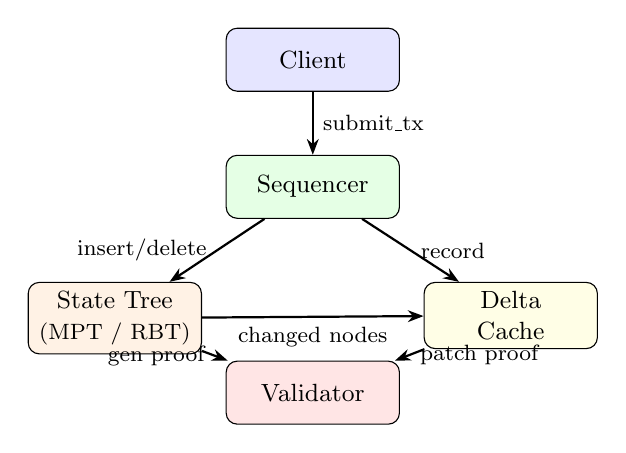
\begin{tikzpicture}[
    node distance=0.8cm and 1.2cm,
    box/.style={draw, rounded corners, minimum width=2.2cm, minimum height=0.8cm, align=center, font=\small},
    arr/.style={-{Stealth[length=2mm]}, thick},
  ]
    \node[box, fill=blue!10] (client) {Client};
    \node[box, fill=green!10, below=of client] (seq) {Sequencer};
    \node[box, fill=orange!10, below left=0.8cm and 0.3cm of seq] (tree) {State Tree\\{\footnotesize (MPT / RBT)}};
    \node[box, fill=yellow!10, below right=0.8cm and 0.3cm of seq] (cache) {Delta\\Cache};
    \node[box, fill=red!10, below=1.8cm of seq] (val) {Validator};

    \draw[arr] (client) -- node[right, font=\footnotesize] {submit\_tx} (seq);
    \draw[arr] (seq) -- node[left, font=\footnotesize] {insert/delete} (tree);
    \draw[arr] (seq) -- node[right, font=\footnotesize] {record} (cache);
    \draw[arr] (tree) -- node[below, font=\footnotesize] {changed nodes} (cache);
    \draw[arr] (cache) -- node[right, font=\footnotesize] {patch proof} (val);
    \draw[arr] (tree) -- node[left, font=\footnotesize] {gen proof} (val);
  \end{tikzpicture}
  \caption{System architecture. The Sequencer processes batched transactions, updating the State Tree and recording deltas. The Validator verifies proofs, using the Delta Cache to patch stale proofs.}
  \label{fig:architecture}
\end{figure}

The transaction flow proceeds as follows:
a client submits an order operation (insert or delete) to the Sequencer, which enqueues it in a thread-safe deque.
When \texttt{process\_batch} is called, the Sequencer drains the queue under a state lock and applies each transaction to the tree.
After each mutation, the Delta Cache's \texttt{record\_transition} method captures the list of changed node hashes from the tree.
Proof requests are served under the same state lock to guarantee consistency between the returned proof and version number.

\subsection{Merkle-Prefix Tree}

Our Merkle-prefix trie is a Patricia-compressed~\cite{morrison1968patricia} binary trie keyed on the 64-bit big-endian representation of price levels.
Each node stores a compressed \emph{prefix} (a tuple of bits shared by all keys in its subtree) and a Merkle hash.
Leaf nodes additionally store the order value.

\paragraph{Patricia compression.}
Single-child chains are collapsed into the parent node's prefix, ensuring that the trie depth is $O(\log N)$ rather than the full 64-bit key width.
When a new key diverges within an existing node's prefix, the node is split at the divergence point.

\paragraph{Merkle hashing.}
We use domain-separated SHA-256~\cite{merkle1988digital}: leaf hashes are computed as $H(\texttt{0x00} \| \mathit{key} \| \mathit{value})$ and internal hashes as $H(\texttt{0x01} \| H_{\mathrm{left}} \| H_{\mathrm{right}})$.
The domain separation prefix prevents second-preimage attacks that could confuse leaf data with internal node structure.

\paragraph{Proof generation.}
To generate an inclusion proof for a key, the algorithm walks from the root to the target leaf, collecting the sibling hash at each internal node along the path.
Because the trie depth is $O(\log N)$ after Patricia compression, proof generation is $O(\log N)$.

\paragraph{Change tracking.}
After each insert or delete, the tree records \texttt{(old\_hash, new\_hash)} pairs for every node whose hash changed, enabling the delta cache to track mutations without additional tree traversal.

\subsection{Red-Black Tree}

Our Red-Black Tree~\cite{cormen2009introduction} is a standard self-balancing BST augmented with per-node Merkle hashes.
Structural operations (insert, delete, search) are $O(\log N)$, including the hash propagation along the path from the affected node to the root after rotations.

\paragraph{The proof generation bottleneck.}
Unlike the Merkle-prefix trie, the Red-Black Tree's binary search structure does not correspond to a Merkle tree structure.
To generate an inclusion proof, the implementation must:
\begin{enumerate}
  \item Perform an in-order traversal to collect all $N$ leaf data hashes.
  \item Build a temporary balanced Merkle tree (a flat array of size $2N$) over the sorted hashes.
  \item Locate the target key's position in the sorted order.
  \item Extract sibling hashes along the path from the target leaf to the root of the temporary tree.
\end{enumerate}
Steps 1 and 2 are each $O(N)$, making the overall proof generation $O(N)$.
Root-hash computation similarly requires the full traversal and temporary tree construction.

\subsection{Aardvark Delta Cache}

The delta cache stores a sequence of \texttt{Delta} records, each containing a version number, the old and new root hashes, a list of changed node-hash pairs, and a timestamp.

\paragraph{Recording.}
After each tree mutation, the Sequencer calls \texttt{record\_transition}, which reads the tree's changed-node list and creates a new \texttt{Delta} at the next version.

\paragraph{Proof patching.}
Given a stale proof generated at version $V_1$ and a target version $V_2$, the \texttt{patch\_proof} method iterates through the delta chain from $V_1 + 1$ to $V_2$.
For each delta, it scans the proof's sibling hashes and replaces any that match an \texttt{old\_hash} with the corresponding \texttt{new\_hash}.
The complexity is $O(D \cdot P \cdot C)$, where $D = V_2 - V_1$ is the version gap, $P$ is the proof length, and $C$ is the average number of changed nodes per version.
Critically, this cost is independent of $N$.

\paragraph{Garbage collection.}
The cache supports a \texttt{prune(keep\_last)} method that removes deltas older than a configurable retention window to bound memory consumption.

The delta cache is \emph{tree-agnostic}: it depends only on the \texttt{StateTree} interface (\texttt{get\_root\_hash} and \texttt{get\_changed\_nodes}).
This means it benefits both tree types, though the benefit is asymmetric: for the Red-Black Tree, patching avoids an $O(N)$ regeneration, while for the Merkle-prefix trie, it avoids only an $O(\log N)$ regeneration.

% ------------------------------------------------------------------
% 4  EVALUATION
% ------------------------------------------------------------------
\section{Evaluation}
\label{sec:eval}

\subsection{Experimental Setup}

All experiments were conducted on a MacBook Pro with an Apple M4 chip (10 cores: 4 performance, 6 efficiency), 16~GB of RAM, running macOS.
The prototype is implemented in Python~3.13 (1{,}689 lines of production code) using SHA-256 from the standard library's \texttt{hashlib} module.
We use \texttt{pytest-benchmark}~4.0 for timing measurements and \texttt{tracemalloc} for memory profiling.

Each benchmark inserts $N$ randomly generated keys (uniform distribution over a range of $100N$, seeded for reproducibility) into a fresh tree.
We report results for $N \in \{100,\; 1{,}000,\; 10{,}000\}$.

\subsection{Insert Throughput}

Table~\ref{tab:insert} shows the total time to insert $N$ keys into each tree type.
For the Red-Black Tree, we measure the structural insert (BST insertion, RB fix-up, per-node hash propagation) with a single final Merkle commitment at the end, which is the practical configuration for batch loading.

\begin{table}[t]
  \centering
  \caption{Total insert time for $N$ keys (ms).}
  \label{tab:insert}
  \begin{tabular}{@{}rrrr@{}}
    \toprule
    $N$ & MPT & RBT & Ratio \\
    \midrule
    100    & 0.93  & 0.85  & 1.09$\times$ \\
    1{,}000  & 11.72 & 14.42 & 0.81$\times$ \\
    10{,}000 & 141.13 & 190.83 & 0.74$\times$ \\
    \bottomrule
  \end{tabular}
\end{table}

At small sizes ($N = 100$), the Red-Black Tree is marginally faster due to simpler node allocation.
As $N$ grows, the Merkle-prefix trie's $O(\log N)$-per-key insert (which includes incremental Merkle rehashing) becomes competitive: at $N = 10{,}000$, it is 26\% faster than the RBT even when the RBT defers its $O(N)$ Merkle commitment to a single final call.

\subsection{Proof Generation Latency}

Table~\ref{tab:proof} and Figure~\ref{fig:proof_gen} present the central result: proof generation latency for a single randomly selected key.

\begin{table}[t]
  \centering
  \caption{Single-key proof generation latency ($\mu$s).}
  \label{tab:proof}
  \begin{tabular}{@{}rrrr@{}}
    \toprule
    $N$ & MPT & RBT & Speedup \\
    \midrule
    100      & 6.23   & 77.20      & 12$\times$ \\
    1{,}000    & 7.15   & 729.66     & 102$\times$ \\
    10{,}000   & 7.21   & 9{,}487.03   & 1{,}316$\times$ \\
    \bottomrule
  \end{tabular}
\end{table}

\begin{figure}[t]
  \centering
  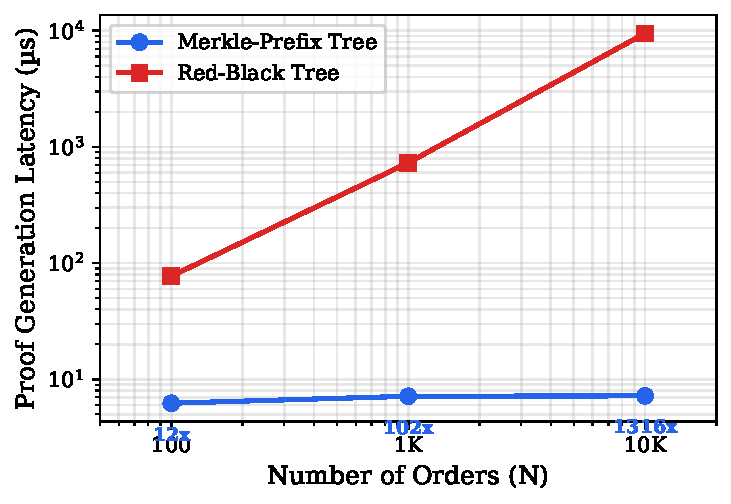
\includegraphics[width=\columnwidth]{figures/proof_generation.pdf}
  \caption{Proof generation latency vs.\ order book size. The Merkle-prefix trie (blue) remains nearly flat ($O(\log N)$) while the Red-Black Tree (red) scales linearly.}
  \label{fig:proof_gen}
\end{figure}

The Merkle-prefix trie's proof generation is nearly constant (6--7~$\mu$s), reflecting the $O(\log N)$ path length with Patricia compression.
The Red-Black Tree's latency scales linearly from 77~$\mu$s at $N = 100$ to 9.5~ms at $N = 10{,}000$, confirming the $O(N)$ in-order traversal and temporary Merkle tree construction.
At $N = 10{,}000$, the trie is \textbf{1{,}316$\times$ faster}.

This result has direct implications for sequencer throughput: a sequencer serving 1{,}000 proof requests per second against a 10{,}000-order book would spend 9.5~seconds per batch on RBT proofs but only 7.2~ms with the trie.

\subsection{Delta Cache Effectiveness}

Table~\ref{tab:delta} compares the cost of patching a stale proof via the delta cache (after $D = 10$ intervening mutations) against full proof regeneration on the Red-Black Tree.

\begin{table}[t]
  \centering
  \caption{Stale proof recovery: delta-cache patch vs.\ RBT full regeneration ($\mu$s).}
  \label{tab:delta}
  \begin{tabular}{@{}rrrr@{}}
    \toprule
    $N$ & Patch & RBT Regen & Speedup \\
    \midrule
    100      & 7.52   & 77.20      & 10$\times$ \\
    1{,}000    & 9.92   & 729.66     & 74$\times$ \\
    10{,}000   & 10.38  & 9{,}487.03   & 914$\times$ \\
    \bottomrule
  \end{tabular}
\end{table}

\begin{figure}[t]
  \centering
  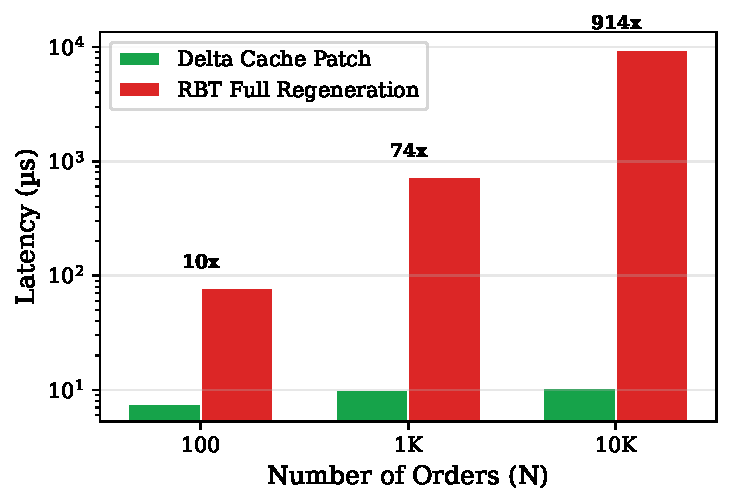
\includegraphics[width=\columnwidth]{figures/delta_cache_speedup.pdf}
  \caption{Delta cache patch time vs.\ Red-Black Tree full proof regeneration. Patching remains nearly constant while regeneration scales linearly with $N$.}
  \label{fig:delta_cache}
\end{figure}

Delta-cache patching takes ${\sim}7$--10~$\mu$s regardless of tree size, consistent with its $O(D \cdot P \cdot C)$ complexity being independent of $N$.
Compared to RBT full regeneration, patching achieves 10$\times$ to 914$\times$ speedup.
For the Merkle-prefix trie, where proof regeneration is already $O(\log N)$ (${\sim}7~\mu$s), the delta cache offers marginal benefit---confirming that the cache's primary value lies in avoiding the RBT's $O(N)$ regeneration cost.

\subsection{Memory Overhead}

Table~\ref{tab:memory} reports peak memory consumption measured via \texttt{tracemalloc}.

\begin{table}[t]
  \centering
  \caption{Peak memory consumption (KB).}
  \label{tab:memory}
  \begin{tabular}{@{}rrrr@{}}
    \toprule
    $N$ & MPT & RBT & Ratio (MPT/RBT) \\
    \midrule
    100      & 101.6    & 34.4     & 2.95$\times$ \\
    1{,}000    & 1{,}671.9  & 322.0    & 5.19$\times$ \\
    10{,}000   & 21{,}668.5 & 5{,}055.8  & 4.29$\times$ \\
    \bottomrule
  \end{tabular}
\end{table}

\begin{figure}[t]
  \centering
  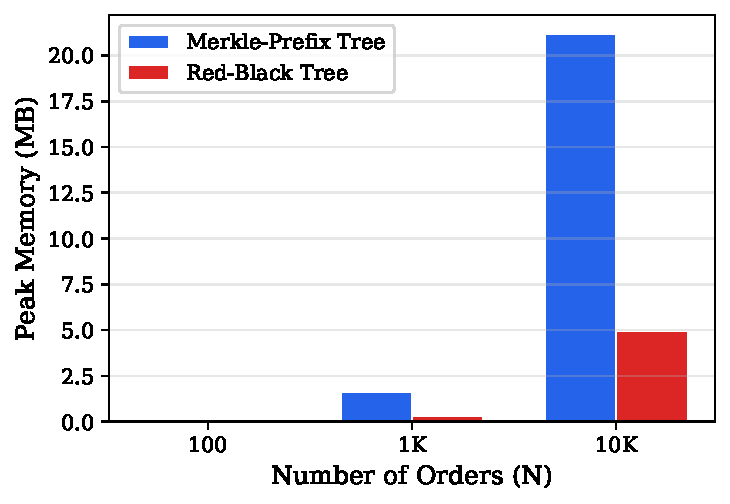
\includegraphics[width=\columnwidth]{figures/memory_comparison.pdf}
  \caption{Peak memory usage. The Merkle-prefix trie uses 3--5$\times$ more memory than the Red-Black Tree due to Python dictionary overhead per trie node.}
  \label{fig:memory}
\end{figure}

The Merkle-prefix trie uses 3--5$\times$ more memory than the Red-Black Tree.
This overhead stems from Python's \texttt{dict} objects used for each trie node's \texttt{children} mapping (with keys 0 and 1), which carry significant per-object overhead compared to the RBT's fixed \texttt{left}/\texttt{right} pointers.
In a production implementation (e.g., Rust or C++), this gap would narrow substantially, as trie nodes could use compact 2-element arrays instead of hash maps.

% ------------------------------------------------------------------
% 5  DISCUSSION
% ------------------------------------------------------------------
\section{Discussion and Limitations}
\label{sec:discussion}

\paragraph{Implementation language.}
Our prototype is implemented in Python, which adds constant-factor overhead from interpreted execution, garbage collection, and object allocation.
While the asymptotic relationships ($O(\log N)$ vs.\ $O(N)$) would be preserved in a systems language, the absolute timings would improve by 10--100$\times$ in Rust or C++.
Notably, the memory overhead gap between the MPT and RBT would also narrow, since a Rust implementation could represent trie node children as a fixed \texttt{[Option<Box<Node>>; 2]} array (16 bytes) versus Python's \texttt{dict} (hundreds of bytes per object).

\paragraph{Key distribution.}
Our benchmarks use uniformly random integer keys.
Real order book price levels are often clustered around the current market price, which could affect trie depth and Patricia compression effectiveness.
An evaluation with realistic order flow data is left as future work.

\paragraph{No ZK-SNARK integration.}
Our proofs are standard Merkle inclusion proofs, not zero-knowledge proofs.
Integrating with a ZK proving system (e.g., StarkEx~\cite{starkware2020starkex}) would require expressing the proof verification logic as an arithmetic circuit, which introduces additional constraints on the choice of hash function and tree structure.

\paragraph{Thread safety.}
The Sequencer uses Python's Global Interpreter Lock (GIL) and explicit \texttt{RLock}/\texttt{Lock} primitives for thread safety.
A production system would require lock-free or sharded designs to achieve true parallelism.

\paragraph{Future work.}
Several directions merit further investigation:
(1)~Verkle trees~\cite{kuszmaul2019verkle}, which use polynomial commitments to achieve $O(1)$-sized proofs;
(2)~integration with ZK proving backends for validity-rollup settlement;
(3)~evaluation with real DEX order flow data from protocols such as dYdX~\cite{dydx2021} or Loopring~\cite{wang2019loopring};
(4)~a Rust reimplementation to eliminate Python-specific overhead and provide production-realistic absolute performance numbers.

% ------------------------------------------------------------------
% 6  CONCLUSION
% ------------------------------------------------------------------
\section{Conclusion}
\label{sec:conclusion}

We have presented a prototype Layer-2 order book matching engine that compares two authenticated data structures---a Patricia-compressed Merkle-prefix trie and a hash-augmented Red-Black Tree---for verifiable state management.
Our benchmarks demonstrate that the Merkle-prefix trie achieves up to 1{,}316$\times$ faster proof generation at $N = 10{,}000$ by eliminating the Red-Black Tree's $O(N)$ in-order traversal and temporary Merkle tree construction.
By integrating an Aardvark-style delta cache, stale proofs can be patched in ${\sim}10~\mu$s regardless of tree size, compared to the 9.5~ms required by full Red-Black Tree proof regeneration---a 914$\times$ speedup at $N = 10{,}000$.
The Merkle-prefix trie trades 3--5$\times$ higher memory usage for its proof generation advantage, a trade-off that would narrow in a systems-language implementation.

These results demonstrate that the choice of authenticated data structure has a profound impact on L2 sequencer performance, and that Merkle-prefix tries combined with delta caching offer a practical path toward high-throughput verifiable order book state.

% ------------------------------------------------------------------
% REFERENCES
% ------------------------------------------------------------------

{\footnotesize
\bibliographystyle{plain}
\bibliography{references}
}

\end{document}
